\documentclass[addpoints,12pt]{exam}
\usepackage{multicol,xy}
\usepackage{graphicx,multicol}
\usepackage[euler-digits]{eulervm}
\usepackage{charter,amsmath,amssymb}
\usepackage[letterpaper,margin=1in]{geometry}
\pagestyle{headandfoot}
\runningheadrule
\firstpageheader{\bf Red Form}{\bf Exam 3}
{\bf 8 April 2015}
\runningheader{\bf Red Form}
{\bf Exam Three, Page \thepage\ of \numpages}
{\bf 8 April 2015}
\firstpagefooter{}{}{}
\runningfooter{}{}{}
\everymath{\displaystyle}
\begin{document}

\begin{questions}

\begin{multicols}{2}
\question[10]
As illustrated at the right,
a UPC~barcode contains a one-digit number
(0 in the example) followed by a five-digit
manufacturer code (36000 in the example)
followed by a five-digit product code
(29145 in the example) followed by a check
digit (2 in the example). How many different
manufacturer codes are possible?
\break\\
\begin{center}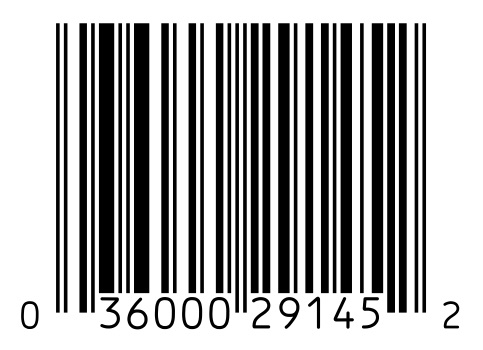
\includegraphics[scale=.5]{Barcode}\end{center}
\end{multicols}

\question[16] Two cards are drawn at random from a deck of playing cards
without replacement.
\begin{parts}
\part What is the probability that both cards are Kings?
\begin{solution}%[1in]
$\frac{4}{52}\cdot\frac{3}{51}=\frac{1}{221}
\approx 0.005$
\end{solution}
\part What is the probability that the second card is a King
given that the first card is a Queen?
\begin{solution}%[1in]
$\frac{4}{51}\approx 0.078$
\end{solution}
\end{parts}

\question[18] The following table lists the numbers
of residents of Iowa between 2008 and 2012 that
spoke languages other than English, organized by
language and age
of the resident.\footnote{Source: {\tt www.census.gov}}
\[\begin{array}{r|rrr|r}
\text{Language}&\text{$5$--$17$}
&\text{$18$--$64$}&\ge 65&\text{Total}\\\hline
\text{Spanish or Spanish Creole}&32,196&75,674&4,114&111,984\\
\text{Other Indo-European}&8,978&29,811&6,530&45,319\\
\text{Asian or Pacific Island}&5,624&27,022&2,255&34,901\\
\text{Other}&2,386&7,874&423&10,683\\\hline
\text{Total}&49,184&140,381&13,322&202,887
\end{array}\]
The row labeled by Other refers to languages
other than English not falling into the categories
listed in the remaining rows.
\begin{parts}
\part How many residents of age $65$ or older
spoke a language other than English?
\begin{solution}%[2cm]
$13,322$
\end{solution}
\part What is the probability that a randomly selected
resident spoke an Asian or Pacific Island language
given that that individual was between $18$ and $64$ years old?
\begin{solution}%[2cm]
$\frac{27022}{140381}\approx 0.192$
\end{solution}
\part What is the probability that a randomly selected
resident that spoke a language other than English
was between $5$ and $17$ years old?
\begin{solution}%[2cm]
$\frac{49184}{202887}\approx 0.242$
\end{solution}
\end{parts}

\question[24] In a recent survey of 884 Americans between the ages
of $18$ and $50$,\\ $120$ reported that they have tattoos,
$72$ have body piercings, and $41$ have both.
\footnote{Source: 2004, American Journal of Dermatology}

\begin{parts}
\part What is the probability that a randomly
selected American has a tattoo?
\begin{solution}%[1.5cm]
$\frac{120}{884}\approx 0.136$
\end{solution}
\part What is the probability that a randomly
selected American has a piercing?
\begin{solution}%[1.5cm]
$\frac{72}{884}\approx 0.081$
\end{solution}
\part What is the probability that a randomly
selected American has a both a tattoo and a piercing?
\begin{solution}%[1.5cm]
$\frac{41}{884}\approx 0.046$
\end{solution}
\part\label{Independent} According to this data do
the decision to get a piercing and the decision
to get a tattoo appear to be independent?
Recall that two events $E$ and $F$ are called {\em independent}
if $P\left(E\right)P\left(F\right)=P\left(E\cap F\right)$.
\begin{solution}%[1.5cm]
No, since $0.136\cdot 0.081\approx 0.011\ne 0.046$
\end{solution}
\part What is the probability that a randomly
selected American has a tattoo given that that individual
has a piercing?
\begin{solution}%[1.5cm]
$\begin{xy}<.5cm,0cm>:
(-1,2)*+!D{\text{T}};
(1,2)*+!D{\text{P}};
(-1,0)*\cir<1cm>{};
(1,0)*\cir<1cm>{};
(0,0)*{41};
(-2,0)*{79};
(2,0)*{31};
(4,0)*{733};
\end{xy}$
\qquad $\frac{41}{72}\approx 0.569$
\end{solution}
\part What is the probability that a randomly
selected American has a piercing given that that individual
does {\bf not} have a tattoo?
\begin{solution}%[1.5cm]
$\frac{31}{31+733}\approx 0.041$
\end{solution}
\end{parts}

\question[16] How many anagrams of the word
{\textsf{Machiavellianism}} are there?
\begin{solution}%[3in]
The number of times each distinct letter appears is
shown in the following table.
\[\begin{array}{r|cccccccccc}
\text{letter}&a&c&e&h&i&l&m&n&s&v\\\hline
\text{frequency}&3&1&1&1&3&2&2&1&1&1
\end{array}\]
Thus the number of anagrams is
\[\frac{16!}{3!3!2!2!}=145,297,152,000.\]
\end{solution}

\vfill
\begin{center}\gradetable[h][questions]\end{center}

\end{questions}
\end{document}
